\section{Лекция 11.04.2020} 

Если у вас ощущение, что в конспекте баг, можете проверить \href{https://www.dropbox.com/s/xsc0pnkmmre2yhe/LA_19-20_osn_Lecture27.svg?dl=0}{снимок доски}, \href{https://youtube.com/watch?v=6WN92vn1HMQ&list=PLEwK9wdS5g0oP4vhnGvQHPSqshML3Ze4P&index=4&t=0s}{запись} и \href{https://www.dropbox.com/s/wnao00nkxnvb9h3/LO_basics.pdf?dl=0}{слайды}.

\subsection{Метрические задачи в $\RR^3$}

\subsubsection{Расстояния то точки $v$ до прямой $l = v_0 + at$}

{
\begin{wrapfigure}[1]{r}{4cm}
    \vspace{-40pt}
    
\includegraphics[height=2.5cm]{lecture27_drawing_1}
\end{wrapfigure}

\begin{equation*}
    \displaystyle
    \rho(v, l) = \frac{\left|[v - v_0, a]\right|}{|a|}
\end{equation*}
}


\subsubsection{Расстояние от точки $v$ до плоскости $P$ с направляющей нормалью $n$ и направляющим подпространством $S$ ($S = n^{\perp}$)}

{
\begin{wrapfigure}{r}{4cm}
    \vspace{-20pt}
    
\includegraphics[height=2.5cm]{lecture27_drawing_2}
\end{wrapfigure}

\begin{equation*}
    \displaystyle
    \rho(v, P) = \left|\ort_S (v - v_0)\right| = \left|\pr_{\left< n \right>} (v - v_0)\right| = \left|\frac{(v - v_0, n)}{(n, n)} n\right| = \frac{|(v - v_0, n)|}{|n|}.
\end{equation*}
\vspace{1cm}
}


\subsubsection{Расстояние между двумя скрещивающимися прямыми $l_1 = v_1 + a_1 t$ и $l_2 = v_2 + a_2 t$}

{
\begin{wrapfigure}{r}{4.5cm}
    \vspace{-10pt}
    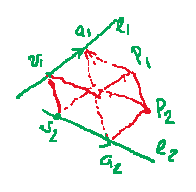
\includegraphics[height=3.5cm]{lecture27_drawing_3}
\end{wrapfigure}

\begin{equation*}
    \begin{gathered}
        p_1 = v_1 + \left< a_1, a_2 \right> \\
        p_2 = v_2 + \left< a_1, a_2 \right> \\
        \rho(l_1, l_2) = \rho(p_1, p_2)
    \end{gathered}
    \hspace{2cm}
    \rho(l_1, l_2) = \frac{\left|(a_1, a_2, v-1 - v_2)\right|}{\left|[a_1, a_2]\right|}
\end{equation*}
\vspace{1.5cm}
}


\subsubsection{Угол между прямой $l$ с направляющим вектором $a$ и плоскостью $P$ с нормалью $n$}

{
\begin{wrapfigure}{r}{6cm}
    \vspace{-10pt}
    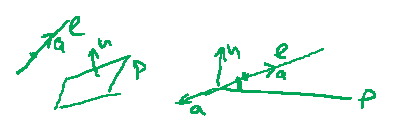
\includegraphics[height=2cm]{lecture27_drawing_4}
\end{wrapfigure}

\begin{equation*}
    \angle(l, P) = \frac{\pi}{2} - \min\left(\angle(a, n), \angle(a, -n)\right)
\end{equation*}
\vspace{0.5cm}
}


\subsubsection{Угол между двумя прямыми $l_1$ с направляющим вектором $a_1$ и $l_2$ с направляющим вектором $a_2$}

{
\begin{wrapfigure}{r}{5cm}
    \vspace{-10pt}
    
\includegraphics[height=1.5cm]{lecture27_drawing_5}
\end{wrapfigure}

\begin{equation*}
    \angle (l_1, l_2) = \min(\angle(a_1, a_2), \angle(a_1, -a_2))
.\end{equation*}
}

\subsubsection{Угол между двумя плоскостями $P_1$ с нормалью $n_1$ и $P_2$ с нормалью $n_2$}

{
\begin{wrapfigure}{r}{4cm}
    \vspace{-10pt}
    
\includegraphics[height=1.5cm]{lecture27_drawing_6}
\end{wrapfigure}

\begin{equation*}
    \angle(P_1, P_2) = \min (\angle(n_1, n_2), \angle(n_1, -n_2))
.\end{equation*}
}


\subsection{Линейные операторы}

Пусть $V$ --- векторное пространство над $F$, $\dim V = n$.

\begin{definition}
\textit{Линейным оператором} (или \textit{линейным преобразованием}) на/в $V$ называется всякое линейное отображение $\phi \colon V \to V$ (то есть из $V$ \underline{\underline{в себя}}).
\end{definition}

$\L(V) := \hom(V, V)$ --- все линейные операторы на/в $V$.


\subsection{Матрица линейного оператора в фиксированном базисе}

Пусть $\phi \in \L(V)$, $\E = (e_1, \dots, e_n)$ --- базис $V$.

Тогда, $(\phi(e_1), \dots, \phi(e_n)) = (e_1, \dots, e_n) \cdot A$, $\quad A \in M_{n}(F)$.

$A$ называется матрицей линейного оператора в базисе $\E$.

Обозначение: $A(\phi, \E)$.

В столбце $A^{(j)}$ записаны координаты вектора $\phi(e_j)$ в базисе $\E$.


\subsection{Примеры линейных операторов}

\begin{enumerate}
    \item (скалярный оператор) $\lambda \in F \leadsto \phi = \lambda \cdot \mathrm{Id}$.

        $\phi(v) = \lambda \cdot v$ для всех $v \in V$.

        Для любого базиса $\E$ имеем $A(\phi, \E) = \lambda \cdot E$.

    \item $V = \RR^2$, $\phi$ --- поворот на угол $\alpha$ (вокруг 0)

        $\E = (e_1, e_2)$ положительно ориентированный ортонормированный базис $\implies A(\phi, \E) = \begin{pmatrix} 
            \cos \alpha & -\sin \alpha \\
            \sin \alpha & \cos \alpha
        \end{pmatrix}$.

    \item $V = F[x]_{\leq n}$, $\phi \colon f \mapsto f'$ (отображение дифференцирования)

        (при $F \neq \RR$ полагают по определению $x^k \mapsto kx^{k - 1}$, $k = 0, \dots, n$)

        Если $\E = (1, x, x^2, \dots, x^{n})$, то $A(\phi, \E) = \begin{pmatrix} 
            0 & 1 & 0 & 0 & \dots & 0 \\
            0 & 0 & 2 & 0 & \dots & 0 \\
            0 & 0 & 0 & 3 & \dots & 0 \\
            \vdots & \vdots & \vdots & \vdots & \ddots & \vdots \\
            0 & 0 & 0 & 0 & \dots & n \\
            0 & 0 & 0 & 0 & \dots & n
        \end{pmatrix}$.
\end{enumerate}


\subsection{Следствия общих фактов о линейных отображениях}

\begin{enumerate}
    \item $\E$ --- базис $V \implies $ отображение $\L(V) \to M_n(F)$, $\phi \mapsto A(\phi, \E)$, является изоморфизмом векторных пространств. В частности:
        \begin{enumerate}[label=\alph*)]
        \item $\phi$ однозначно определяется своей матрицей в любом базисе.
        \item Если $\E$ --- фиксированный базис $V$, то $\forall A \in M_n(F) \ \exists! \phi \in \L(V) : A(\phi, \E) = A$.
        \end{enumerate}

    \item
        $\phi \in \L(V)$, $\E = (e_1, \dots, e_n)$ --- базис $V$, $A = A(\phi, \E)$, 

        \begin{math}
            \begin{cases}
                v = x_1 e_1 + \dots + x_n e_n \\
                \phi(v) = y_1 e_1 + \dots + y_n e_n
            \end{cases} \implies \begin{pmatrix} y_1 \\ \dots \\ y_n \end{pmatrix} = A \cdot \begin{pmatrix} x_1 \\ \dots \\ x_n \end{pmatrix}
        \end{math}

    \item $\E'$ --- другой базис $V$, $\E' = \E \cdot C$, $C \in M_n^{0}(F)$

        $A = A(\phi, \E)$, $A' = A(\phi, \E') \implies A' = C^{-1} A C$.
\end{enumerate}

Следствия из 3:
\begin{enumerate}[label=\alph*)]
    \item $\det A$ не зависит от выбора базиса $\left(\det (C^{-1} A C) = \det A\right)$.
    \item $\tr A$ не зависит от выбора базиса $\left(\tr (C^{-1} A C) = \tr (ACC^{-1}) = \tr A\right)$.
\end{enumerate}


\subsection{Инвариантность определителя и следа матрицы линейного оператора относительно замены базиса}

\begin{comment}
    $\det A$ и $\tr A$ являются инвариантами самого линейного оператора $\phi$.

    Обозначаются: $\det \phi$, $\tr \phi$.
\end{comment}


\subsection{Подобные матрицы, отношение подобия на множестве квадратных матриц фиксированного порядка}

\begin{definition}
    Матрицы $A, A' \in M_n$ называются \textit{подобными}, если $\exists C \in M_n^{0}(F)$, такая что $A' = C^{-1} A C$.
\end{definition}

\begin{comment}
    Отношение подобия является отношением эквивалентности на $M_n(F)$.

    $M_n(F)$ разбивается на классы подобных матриц.
\end{comment}


\subsection{Критерий обратимости линейного оператора в терминах его ядра, образа и определителя}

Пусть $\phi \in \L(V)$.

\begin{proposal}
    Следующие условия эквивалентны:
    \begin{enumerate}[nosep]
    \item $\ker \phi = \{0\}$.
    \item $\Im \phi = V$.
    \item $\phi$ обратима (то есть $\phi$ --- изоморфизм $V$ на себя).
    \item $\det \phi \neq 0$.
    \end{enumerate}
\end{proposal}

\begin{proof}~
    \begin{description}
        \item[$1) \iff 2)$] так как $\dim V = \dim \ker \phi + \dim \Im \phi$. 
        \item[$1) \& 2) \iff 3)$]
        \item[$2) \iff 4)$] $\Im \phi = V \iff \rk \phi = \dim V \iff \det \phi = 0$.
    \end{description}
\end{proof}

\begin{definition}
    Линейный оператор $\phi \in \L(V)$ называется 
    \begin{math}
        \begin{gathered}[t]
            \textit{вырожденным}, \text{ если } \det \phi = 0, \\
            \textit{невырожденным}, \text{ если } \det \phi \neq 0.    
        \end{gathered}
    \end{math}
\end{definition}


\subsection{Подпространства, инвариантные относительно линейного оператора}

\begin{definition}
    Подпространство $U \subseteq V$ называется \textit{инвариантным относительно $\phi$} (или $\phi$-\textit{инвариантным}), \\если $\phi(U) \subseteq U$ (то есть $\phi(u) \in U \ \forall u \in U$).    
\end{definition}

В этой ситуации корректно определён линейный оператор $\phi\Big|_U \colon U \to U$, $u \mapsto \phi(u)$ называется \textit{ограничением} $\phi$ на инвариантное подпространство $U$.


\subsection{Примеры}

\begin{enumerate}
\item Подпространства $\{0\}$ и $V$ всегда $\phi$-инвариантны.
\item $\ker \phi$ --- $\phi$-инвариантно, так как $\phi(\ker \phi) = \{0\} \subseteq \ker \phi$.
\item $\Im \phi$ --- $\phi$-инвариантно, так как $\phi(\Im \phi) \subseteq \phi(V) = \Im \phi$.
\end{enumerate}



\subsection{Наблюдения}

Пусть $\phi \in \L(V)$.

\begin{enumerate}
    \item 
        Пусть $U \subseteq V$ --- $\phi$-инвариантное подпространство, $(e_1, \dots, e_k)$ --- базис $U$, дополним его до базиса $(e_1, \dots, e_n)$ всего $V$.
        
        Тогда $A(\phi, \E)$ имеет вид
        \begin{equation}
            \label{lec27:mat}
            \kbordermatrix{
                  & k & n - k \\
                k & A & B \\
                n - k & 0 & C
            }
        .\end{equation}

        При этом $A\left(\phi\big|_U, (e_1, \dots, e_k)\right) = A$.

        Если
        \begin{math}
            \begin{aligned}[t]
                &U = \ker \phi \implies A = 0, \\
                &U = \Im \phi \implies A = C = 0.
            \end{aligned}
        \end{math}

        Обратно, если для некоторого базиса $\E = (e_1, \dots, e_k) \quad A(\phi, \E)$ имеет вид $\eqref{lec27:mat}$, то векторы $e_1, \dots, e_k$ порождают $\phi$-инвариантное подпространство.

    \item
        Аналогично: $e_{k + 1}, \dots, e_n$ порождают $\phi$-инвариантное подпространство $\iff A(\phi, \E)$ имеет вид
        \begin{equation*}
            \kbordermatrix{
                  & k & n - k \\
                k & A & 0 \\
                n - k & B & C
            }
        .\end{equation*}

    \item 
        Пусть $U_1, U_2 \subseteq V$ --- два $\phi$-инвариантных подпространства, такие что $V = U_1 \oplus U_2$.
        
        Пусть $(e_1, \dots, e_k)$ --- базис $U_1$, $(e_{k + 1}, \dots, e_n)$ --- базис $U_2$.
        Тогда, $\E = (e_1, \dots, e_n)$ --- базис $V$ и $A(\phi, \E)$ имеет вид
        \begin{equation*}
            \kbordermatrix{
                      & k & n - k \\
                k     & \star & 0 \\
                n - k & 0 & \diamond
            }
        .\end{equation*}

    \item
        $A(\phi, \E)$ имеет блочно-диагональный вид
        \begin{center}
            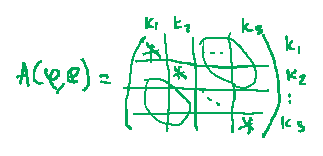
\includegraphics{lecture27_drawing_7}
        \end{center}

        Тогда и только тогда, когда подпространства $U_1, \dots, U_s \ \phi$-инвариантны, где 
        \begin{math}
            \begin{aligned}[t]
                U_1 &= \left<e_1, \dots e_{k_1}\right> \\
                U_2 &= \left< e_{k_1 + 1}, \dots, e_{k_2} \right> \\
                    &\vdots \\
                U_s &= \left< e_{n - k_s + 1}, \dots, e_n \right>
            \end{aligned}
        \end{math}

        Предел мечтаний: найти такой базис $\E$, что $A(\phi, \E)$ диагональна.

        К сожалению, это не всегда возможно.
        \hspace{0.3cm}\raisebox{-0.3cm}{
\includegraphics{lecture27_drawing_8}}
\end{enumerate}
